\documentclass{beamer}
\setbeamerfont{headline}{size=\footnotesize}

\mode<presentation>{
\usetheme{Montpellier}
\setbeamercovered{transparent}
\usecolortheme{lsc}
}

\mode<handout>{
  % tema simples para ser impresso
  \usepackage[bar]{beamerthemetree}
   % Colocando um fundo cinza quando for gerar transparências para serem impressas
  % mais de uma transparência por página
  \beamertemplatesolidbackgroundcolor{black!5}
}

\usepackage{fancyvrb}

\usepackage{amsmath,amssymb}
\usepackage[brazil]{varioref}
\usepackage[english,brazil]{babel}
\usepackage[utf8]{inputenc}
\usepackage{fontawesome5}
\usepackage{ccicons}
\usepackage{makecell} % Adicione isso no preâmbulo do documento

%\usepackage[latin1]{inputenc}
\usepackage{graphicx}
\usepackage{listings}
\usepackage{url}
\usepackage{colortbl}
\usepackage{caption}
\usepackage{transparent}
\usepackage{multirow}
\usepackage{booktabs}
\usepackage{tabularx}
\usepackage{exercise,chngcntr}

\usepackage{xcolor}
\usepackage{tikz}
\usetikzlibrary{shapes, shapes.geometric, arrows.meta, positioning, fit, backgrounds, calc}


% Definição de cores para o código Python
\definecolor{codegreen}{rgb}{0,0.6,0}
\definecolor{codegray}{rgb}{0.5,0.5,0.5}
\definecolor{codepurple}{rgb}{0.58,0,0.82}
\definecolor{backcolour}{rgb}{0.95,0.95,0.92}
% Configuração do estilo do código Python
\lstdefinestyle{mystyle}{
    xleftmargin=0pt,           % Aumenta a margem esquerda
    xrightmargin=10pt,          % Aumenta a margem direita
    frame=single,               % Adiciona um quadro ao redor do código
    framesep=10pt,              % Espaço entre o quadro e o código
    % Outras configurações do lstlisting...
    backgroundcolor=\color{backcolour},
    commentstyle=\color{codegreen},
    keywordstyle=\color{magenta},
    numberstyle=\tiny\color{codegray},
    stringstyle=\color{codepurple},
    basicstyle=\footnotesize\ttfamily,
    breakatwhitespace=false,
    breaklines=true,
    captionpos=b,
    keepspaces=true,
    %numbers=left,
    numbersep=5pt,
    showspaces=false,
    showstringspaces=false,
    showtabs=false,
    tabsize=2,
    basicstyle=\ttfamily, % Usa uma fonte de largura fixa para o código
    upquote=true,         % Tenta usar aspas retas se a fonte suportar,
    breakatwhitespace=false, % Quebra linhas em espaços em branco quando possível
}

\lstset{style=mystyle}

% ------------------------------------------------------------------
% Estilos TikZ reutilizáveis para os diagramas de agente/ambiente
% ------------------------------------------------------------------
\usetikzlibrary{decorations.pathreplacing}
\tikzset{
  agentbox/.style={draw, thick, rounded corners, fill=blue!6, minimum width=3.4cm, minimum height=3.1cm, align=center},
  envbox/.style={draw, thick, rounded corners, fill=green!8, minimum width=1.6cm, minimum height=3.1cm, align=center, rotate=90},
  procnode/.style={draw, thick, rounded corners, fill=white, minimum width=2.6cm, minimum height=0.9cm, align=center, font=\small},
  ovalnode/.style={draw, thick, rounded corners=6pt, fill=orange!10, minimum width=2.6cm, minimum height=0.8cm, align=center, font=\scriptsize},
  flowarrow/.style={-{Latex[length=2.2mm]}, thick},
}

% Comando genérico para os slides de comparação de propriedades de ambientes
% Uso: \comparediagram{ícone esq.}{título esq.}{exemplo esq.}{ícone dir.}{título dir.}{exemplo dir.}{cor esq.}{cor dir.}
\newcommand{\comparediagram}[8]{%
\begin{center}
\begin{tikzpicture}
  \node[draw, thick, rounded corners, fill=#7!12, text width=3.2cm, minimum height=2.6cm, align=center, inner sep=4pt] (left) at (0,0) {\LARGE\color{#7!80!black}#1\\[3pt]\scriptsize\textbf{#2}\\[1pt]{\tiny#3}};
  \node[draw, thick, rounded corners, fill=#8!12, text width=3.2cm, minimum height=2.6cm, align=center, inner sep=4pt] (right) at (4.0,0) {\LARGE\color{#8!80!black}#4\\[3pt]\scriptsize\textbf{#5}\\[1pt]{\tiny#6}};
  \node[draw, circle, fill=white, thick, font=\bfseries\scriptsize] at ($(left)!0.5!(right)$) {VS};
\end{tikzpicture}
\end{center}%
}

\beamertemplatetransparentcovereddynamic
\addtobeamertemplate{title page}{\centering{ 
\includegraphics[width=1.25cm]{figs/logo.png}}}{}
\title[]{Inteligência Artificial}
\author[Elton Sarmanho]{ 
Professor: Elton Sarmanho\inst{1} 
\newline
E-mail: \href{mailto:eltonss@ufpa.br}{eltonss@ufpa.br}\newline
\href{https://github.com/eltonsarmanho}{\faGithub} \href{https://www.linkedin.com/in/elton-sarmanho-836553185/}{\faLinkedin}\\
\ccbyncsa
}   
  \institute[UFRailwayPA]{
   \inst{1}%
     Faculdade de Sistemas de Informação - UFPA/CUNTINS
     }     
 
% Se comentar a linha abaixo, irá aparecer a data quando foi compilada a apresentação  
\date{\today}
\pgfdeclareimage[height= 1.25 cm]{inf}{figs/logo.png}
% pode-se colocar o LOGO assim
\logo{{\transparent{0.35}\pgfuseimage{inf}}}

% \AtBeginSection[]{
%   \begin{frame}<beamer>
%     \frametitle{Roteiro}
%     \tableofcontents[currentsection,currentsubsection]
%   \end{frame}  
% }

\setbeamertemplate{navigation symbols}{\insertframenavigationsymbol \insertsectionnavigationsymbol \insertbackfindforwardnavigationsymbol} 


\expandafter\def\expandafter\insertshorttitle\expandafter{%
  \insertshorttitle\hfill%
  \insertframenumber\,/\,\inserttotalframenumber}
  \renewcounter{Exercise}[section]
  \newcounter{Example}



\begin{document}

\setbeamertemplate{logo}{}
\begin{frame}
\titlepage
\end{frame}
%Começar mostrar Logo apos slide de titulo
\logo{{\transparent{0.35}\pgfuseimage{inf}}}

\begin{frame}
\frametitle{Roteiro}
\tableofcontents[sections={1-3}]
\end{frame}

\begin{frame}{Licença}
    Este trabalho está licenciado sob a licença Creative Commons:

    \bigskip
    \ccbyncsa
\end{frame}
%Declaração das Imagens da Apresentação

%%%%%%%%%%%%%%%%%%%%%%%%%%%%%%%%%%%%%%%%
\section{Planejamento}

\begin{frame}
\frametitle{Nesta aula}
\begin{itemize}
 \item O que é Inteligência Artificial, afinal? Vamos ver as diferentes formas de defini-la e por que essa definição ainda gera debate.
 \item Um panorama histórico: de onde a área veio e para onde está indo.
 \item O conceito central do curso: \textbf{agentes inteligentes}: como são definidos, o que os torna racionais e como se estruturam internamente.
 \item Exemplos de código ficam disponíveis em dois repositórios:
 \begin{itemize}
    \item Do livro-texto: \url{https://github.com/aimacode}
    \item Da disciplina (professor): \faGithub\ \url{https://github.com/eltonsarmanho}
 \end{itemize}
\end{itemize}
\end{frame}
\section{Fundamentação}
\subsection{Conceitos Fundamentais}
\begin{frame}
\centering
\Huge
\textbf{Conceitos\\ Fundamentais}
\end{frame}

\begin{frame}
\frametitle{O que é Inteligência Artificial?}
\small
\begin{itemize}
    \item Não existe uma definição única e consensual de IA, e isso não é um defeito, é um reflexo de que a própria noção de ``inteligência'' já é escorregadia mesmo quando falamos de seres humanos.
    \item A definição de Russell \& Norvig, que seguimos neste curso, é operacional:
    \begin{itemize}
     \item \textbf{IA é o estudo de agentes que recebem percepções do ambiente e executam ações} de modo a maximizar uma medida de desempenho.
    \end{itemize}
    \item Essa definição desloca o foco de ``o que é pensar'' para ``o que o sistema faz'', e é por isso que o conceito de \textbf{agente} será o fio condutor de todo o curso.
    \item IA é, na prática, um guarda-chuva de subcampos: aprendizado de máquina, visão computacional, processamento de linguagem natural, robótica, planejamento, raciocínio sob incerteza, entre outros.
\end{itemize}
\end{frame}

\begin{frame}
\frametitle{Quatro Formas de Encarar a IA}
\begin{itemize}
    \item Historicamente, as tentativas de definir IA se organizam em duas perguntas independentes:
    \begin{itemize}
        \item O sistema deve \textbf{pensar} ou \textbf{agir}?
        \item O padrão de comparação é o \textbf{ser humano} ou um ideal de \textbf{racionalidade}?
    \end{itemize}
    \item Cruzando essas duas perguntas obtemos quatro escolas de pensamento, que vamos percorrer a seguir.
\end{itemize}
\begin{center}
\begin{tabular}{@{}ll@{}}
\toprule
 & \textbf{Padrão: Humano} \quad\quad \textbf{Padrão: Racionalidade} \\
\midrule
\textbf{Pensar} & Pensar Humanamente \quad\ Pensar Racionalmente \\
\textbf{Agir}   & Agir Humanamente \quad\quad\ \ Agir Racionalmente \\
\bottomrule
\end{tabular}
\end{center}
\end{frame}

\begin{frame}
\frametitle{Pensar Humanamente: a Abordagem Cognitiva}
\footnotesize
\begin{itemize}
    \item A ideia aqui é literal: construir programas cujo \textit{funcionamento interno} imite o raciocínio humano, não apenas o resultado final.
    \item Isso exige evidência empírica de como a mente funciona, obtida por introspecção, experimentos psicológicos e, mais recentemente, neuroimagem. É essa ambição que deu origem à \textbf{ciência cognitiva}.
    \item Exemplo clássico: o \textbf{GPS} (\textit{General Problem Solver}, Newell e Simon, 1961) não só resolvia problemas, buscava reproduzir o \textit{traço} de passos que humanos seguem ao resolvê-los.
\end{itemize}
\vspace{-2pt}
\begin{center}
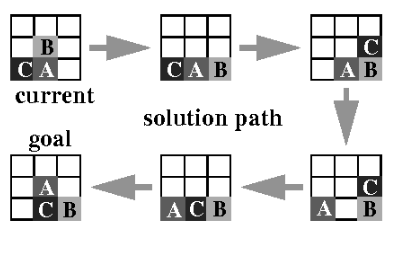
\includegraphics[width=0.34\textwidth]{figs/GPS.png}
\end{center}
\end{frame}

\begin{frame}
\frametitle{Pensar Racionalmente: as Leis do Pensamento}
\footnotesize
\begin{itemize}
    \item Tradição que remonta a Aristóteles: especificar padrões de raciocínio inquestionavelmente corretos, os \textbf{silogismos}, e mecanizá-los.
    \item Deu origem à lógica formal do século XIX e, depois, aos primeiros programas capazes de provar teoremas a partir de premissas.
    \item \textbf{Duas dificuldades}: nem todo conhecimento cotidiano é fácil de formalizar (pense em incerteza), e, mesmo formalizado, resolver o problema pode ser computacionalmente inviável na prática.
\end{itemize}
\vspace{-2pt}
\begin{center}
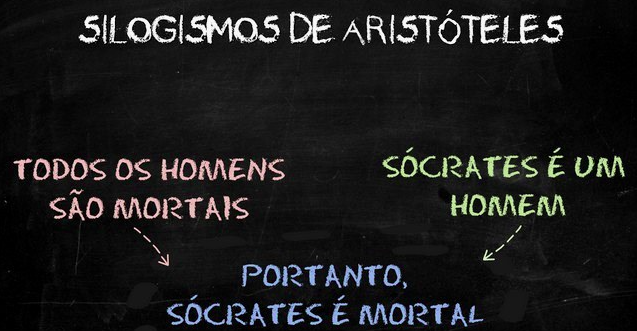
\includegraphics[width=0.4\textwidth]{figs/silogismo.png}
\end{center}
\end{frame}

\begin{frame}
\frametitle{Agir Humanamente: o Teste de Turing}
\footnotesize
\begin{itemize}
    \item Alan Turing propôs, em 1950, contornar ``máquinas podem pensar?'' com um critério comportamental: o \textbf{Jogo da Imitação}.
    \item Um interrogador conversa, por texto, com um humano e com uma máquina sem saber qual é qual, e se não conseguir distingui-los, a máquina é aprovada.
    \item Isso exigiria PLN, representação de conhecimento, raciocínio automatizado e aprendizado de máquina.
    \item \textbf{Reflexão}: LLMs hoje conversam de forma fluente. Isso significa que ``pensam''? O próprio Turing notava que o teste mede comportamento, não mecanismo interno.
\end{itemize}
\vspace{-2pt}
\begin{center}
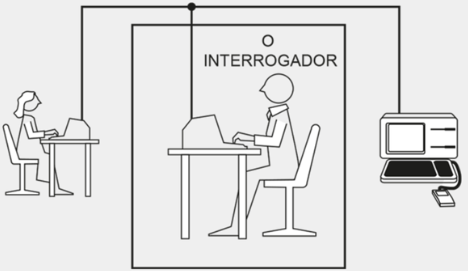
\includegraphics[width=0.3\textwidth]{figs/Turing.png}
\end{center}
\end{frame}

\begin{frame}
\frametitle{Agir Racionalmente: o Agente Racional}
\begin{itemize}
    \item Um \textbf{agente racional} é aquele que age de modo a alcançar o melhor resultado esperado, dado o que percebeu e o que sabe.
    \item Essa noção é \textbf{mais geral} que as leis do pensamento: raciocinar corretamente é apenas \textit{um dos meios} de agir racionalmente, pois às vezes a ação certa nem exige inferência lógica (um reflexo bem calibrado também pode ser racional).
    \item É também \textbf{mais tratável cientificamente} do que imitar humanos: dá para formalizar matematicamente o que é uma boa decisão e construir agentes que se aproximem dela, mesmo quando a solução ótima exata é computacionalmente inviável.
    \item Por essas razões, é a abordagem adotada neste curso, e por isso o restante da disciplina gira em torno do conceito de \textbf{agente}.
\end{itemize}
\end{frame}

\begin{frame}
\frametitle{Resumo das Quatro Abordagens}
\begin{center}
\small
\begin{tabular}{@{}p{2.3cm}p{6.9cm}@{}}
\toprule
\textbf{Abordagem} & \textbf{Ideia central} \\
\midrule
Pensar Humanamente & Reproduzir o processo cognitivo humano (ciência cognitiva) \\
\addlinespace
Pensar Racionalmente & Formalizar o raciocínio correto em lógica (leis do pensamento) \\
\addlinespace
Agir Humanamente & Imitar o comportamento humano de forma indistinguível (Teste de Turing) \\
\addlinespace
Agir Racionalmente & Escolher a melhor ação esperada, dado o conhecimento disponível \\
\bottomrule
\end{tabular}
\end{center}
\bigskip
\centering \textit{Este curso adota a abordagem de \textbf{agentes racionais}.}
\end{frame}



\begin{frame}
\frametitle{Áreas de Apoio para IA}
\begin{figure}
 \centering
 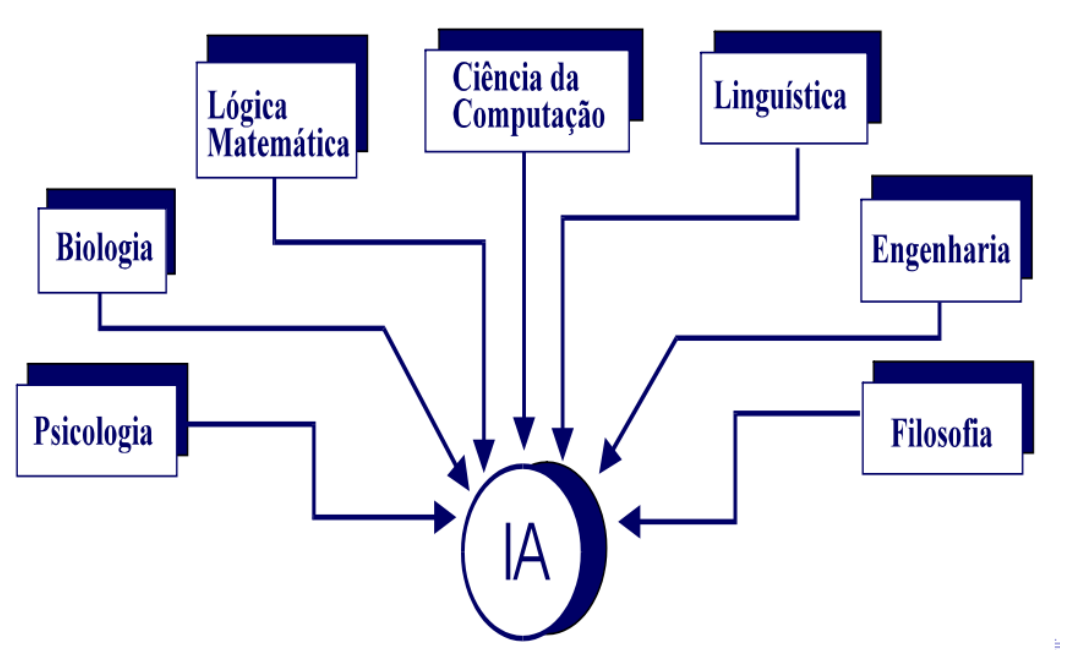
\includegraphics[width=1\textwidth]{figs/areasApoioIA.png}
 \end{figure}
\end{frame}

\begin{frame}
\frametitle{Sub-Áreas da IA}
\begin{figure}
 \centering
 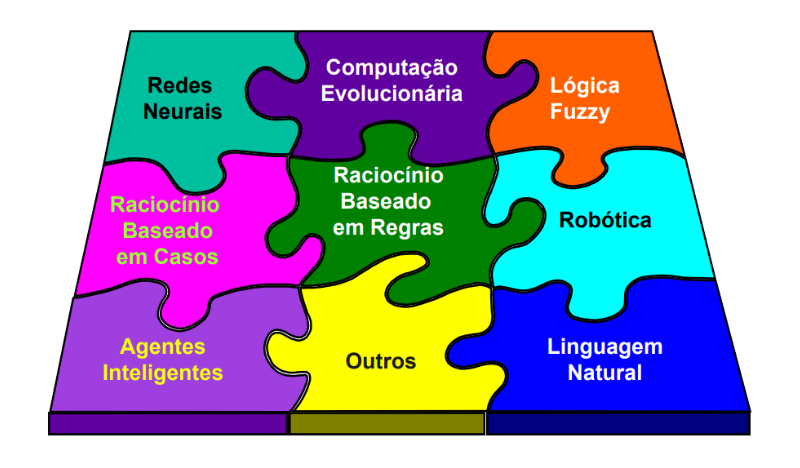
\includegraphics[width=1\textwidth]{figs/subareasIA.png}
 \end{figure}
\end{frame}


\subsection{Contexto Histórico}
\begin{frame}
\frametitle{Linha do Tempo}

\begin{figure}
 \centering
 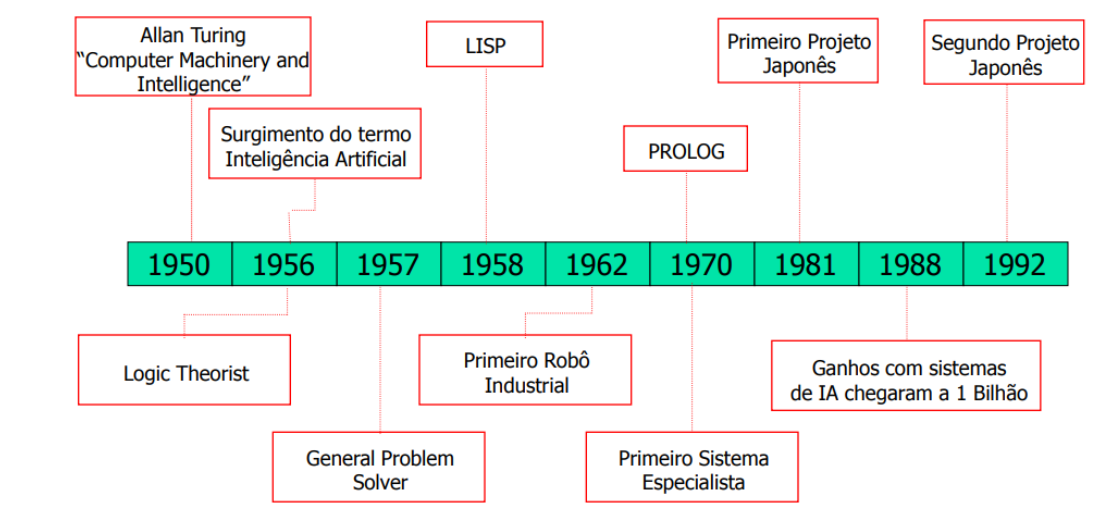
\includegraphics[width=1\textwidth]{figs/linhaDoTempo.png}
 \end{figure}
\end{frame}
\begin{frame}
\frametitle{Gestação da IA (1943–1955)}
\scriptsize
\begin{columns}[T]
\begin{column}{0.58\textwidth}
\begin{itemize}
    \item McCulloch e Pitts (1943) propõem o primeiro modelo matemático de neurônio artificial.
    \item Hebb (1949) propõe a regra de aprendizagem que leva seu nome, ainda usada hoje.
    \item Minsky e Edmonds constroem o SNARC (1951), o primeiro computador neural.
\end{itemize}
\end{column}
\begin{column}{0.38\textwidth}

\includegraphics[width=0.8\textwidth]{img/neuronio_artificial_mcculloch_pitts.png}
\end{column}
\end{columns}
\end{frame}

\begin{frame}
\frametitle{Nascimento da IA (1956)}
\footnotesize
\begin{columns}[T]
\begin{column}{0.6\textwidth}
\begin{itemize}
    \item McCarthy organiza o workshop de Dartmouth, o marco fundador da área.
    \item É ali que o termo \textbf{``Inteligência Artificial''} é cunhado.
    \item Participam nomes como Minsky, Shannon e Newell.
\end{itemize}
\end{column}
\begin{column}{0.35\textwidth}
\centering
{\Huge\faUniversity}
\end{column}
\end{columns}
\end{frame}

\begin{frame}
\frametitle{Entusiasmo Inicial (1952–1969)}
\footnotesize
\begin{columns}[T]
\begin{column}{0.6\textwidth}
\begin{itemize}
    \item O \textbf{Logic Theorist} e o \textbf{GPS} provam teoremas e resolvem problemas como humanos.
    \item Arthur Samuel cria um programa de damas que aprende jogando contra si mesmo.
\end{itemize}
\end{column}
\begin{column}{0.35\textwidth}
\centering
{\Huge\faChessKnight}
\end{column}
\end{columns}
\end{frame}

\begin{frame}
\frametitle{O Retorno das Redes Neurais (1986–presente)}
\footnotesize
\begin{columns}[T]
\begin{column}{0.58\textwidth}
\begin{itemize}
    \item A \textbf{retropropagação} é redescoberta, permitindo treinar redes com várias camadas.
    \item Reacende o confronto entre IA simbólica e IA conexionista.
\end{itemize}
\end{column}
\begin{column}{0.38\textwidth}
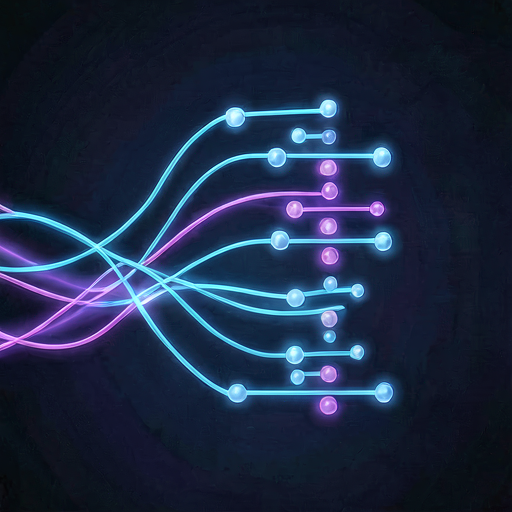
\includegraphics[width=\textwidth]{img/rede_neural_profunda.png}
\end{column}
\end{columns}
\end{frame}

\begin{frame}
\frametitle{Método Científico e Big Data (1987–2012)}
\footnotesize
\begin{columns}[T]
\begin{column}{0.6\textwidth}
\begin{itemize}
    \item A IA passa a exigir \textbf{rigor experimental}, aproximando-se de estatística e otimização.
    \item Com o \textbf{ImageNet} e GPUs, o \textbf{AlexNet} (2012) inicia a revolução do deep learning.
\end{itemize}
\end{column}
\begin{column}{0.35\textwidth}
\centering
{\Huge\faDatabase}
\end{column}
\end{columns}
\end{frame}

\begin{frame}
\frametitle{A Era dos Transformers e dos LLMs (2017–presente)}
\footnotesize
\begin{columns}[T]
\begin{column}{0.58\textwidth}
\begin{itemize}
    \item ``Attention Is All You Need'' (2017) introduz o \textbf{Transformer}, base dos grandes modelos de linguagem.
    \item O ChatGPT (2022) populariza os \textbf{LLMs}, tornando a IA conversacional cotidiana.
\end{itemize}
\end{column}
\begin{column}{0.38\textwidth}

\includegraphics[width=\textwidth]{img/transformer_llm_atencao.png}
\end{column}
\end{columns}
\end{frame}

\subsection{Estado da Arte}
\begin{frame}
\frametitle{O que está em alta agora}
\begin{itemize}
    \item A IA já teve muitos marcos históricos (Deep Blue, DART, Remote Agent). O foco aqui é outro: o que domina o noticiário e a pesquisa \textbf{hoje}.
    \item Quatro frentes concentram praticamente todo o hype atual: carros autônomos, LLMs, geração de conteúdo e agentes de IA.
\end{itemize}
\end{frame}

\begin{frame}
\frametitle{Condução Autônoma}
\footnotesize
\begin{columns}[T]
\begin{column}{0.6\textwidth}
\begin{itemize}
    \item Waymo e Cruise já operam frotas de táxis \textbf{sem motorista} em várias cidades dos EUA.
    \item Tesla e outras montadoras oferecem condução assistida cada vez mais autônoma em carros comerciais.
\end{itemize}
\end{column}
\begin{column}{0.35\textwidth}
\centering
{\Huge\faCarSide}
\end{column}
\end{columns}
\end{frame}

\begin{frame}
\frametitle{Modelos de Linguagem (LLMs)}
\footnotesize
\begin{columns}[T]
\begin{column}{0.58\textwidth}
\begin{itemize}
    \item \textbf{GPT}, \textbf{Gemini} e \textbf{Claude} conversam, programam, resumem e traduzem com alta fluência.
    \item Limitações a lembrar: \textbf{alucinações}, vieses herdados dos dados e alto custo computacional.
\end{itemize}
\end{column}
\begin{column}{0.38\textwidth}

\includegraphics[width=\textwidth]{img/transformer_llm_atencao.png}
\end{column}
\end{columns}
\end{frame}

\begin{frame}
\frametitle{Geração de Imagem e Vídeo por IA}
\footnotesize
\begin{columns}[T]
\begin{column}{0.58\textwidth}
\begin{itemize}
    \item Modelos de difusão (Midjourney, Sora e sucessores) geram imagens e vídeos realistas a partir de texto.
    \item Levanta questões novas: direitos autorais, \textit{deepfakes} e verificação de autenticidade.
\end{itemize}
\end{column}
\begin{column}{0.38\textwidth}
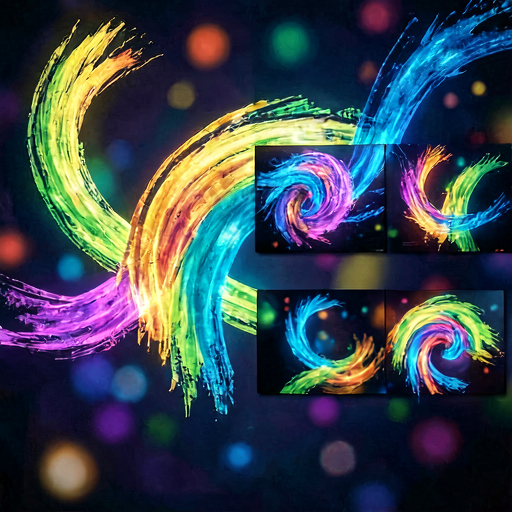
\includegraphics[width=\textwidth]{img/geracao_conteudo_ia.png}
\end{column}
\end{columns}
\end{frame}

\begin{frame}
\frametitle{Agentes de IA: do Texto à Ação}
\footnotesize
\begin{columns}[T]
\begin{column}{0.58\textwidth}
\begin{itemize}
    \item A fronteira atual: transformar um LLM em \textbf{agente}, que lê, decide e age (chama ferramentas, executa código, navega na web).
    \item LangChain e LangGraph orquestram esse ciclo, formando um \textbf{agente} no sentido de Russell \& Norvig.
\end{itemize}
\end{column}
\begin{column}{0.35\textwidth}
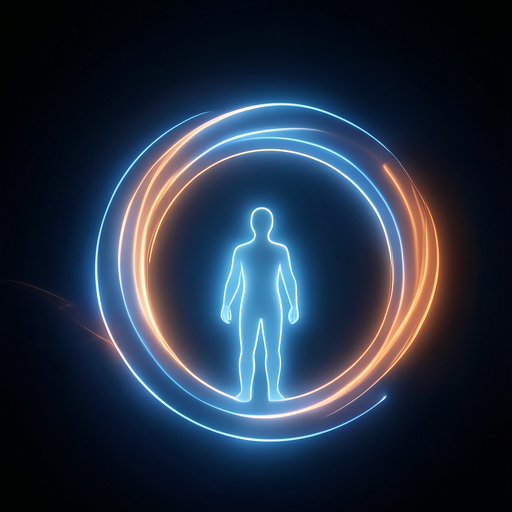
\includegraphics[width=\textwidth]{img/agente_percepcao_decisao_acao.png}
\end{column}
\end{columns}
\end{frame}

\begin{frame}
\frametitle{Conclusão}
\begin{itemize}
    \item O fio que conecta todo o hype atual é sempre o mesmo conceito: um sistema que \textbf{percebe} um ambiente e \textbf{age} sobre ele para atingir um objetivo.
    \item É exatamente esse conceito, o de \textbf{agente}, que vamos formalizar na próxima parte da aula.
\end{itemize}
\end{frame}

\section{Agentes Inteligentes}
\subsection{Conceitos Fundamentais}
\begin{frame}
\centering
\Huge
\textbf{Agentes\\Inteligentes}
\end{frame}

\begin{frame}
\frametitle{Uma Analogia antes da Formalização}
\footnotesize
\begin{columns}[T]
\begin{column}{0.4\textwidth}
\begin{figure}
 \centering
 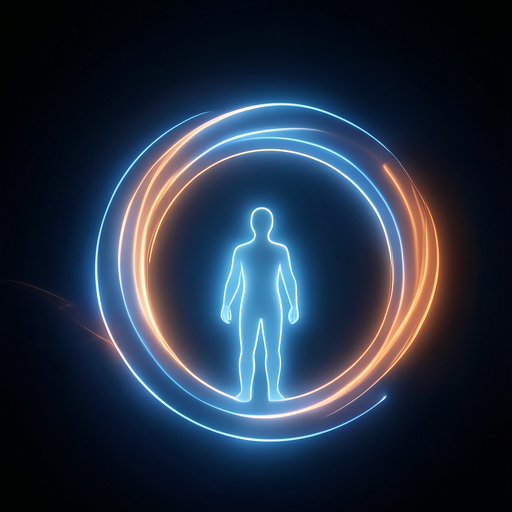
\includegraphics[width=\textwidth]{img/agente_percepcao_decisao_acao.png}
 \caption{\scriptsize Metáfora de um agente: um fluxo entra (percepção), atravessa a figura (decisão) e sai como ação, em ciclo contínuo com o ambiente.}
\end{figure}
\end{column}
\begin{column}{0.56\textwidth}
\begin{itemize}
    \item Antes de formalizar, vale fixar a intuição: um agente é qualquer coisa que \textbf{percebe} seu entorno e \textbf{age} sobre ele, de forma contínua, seja um robô, um termostato ou um programa.
\end{itemize}
\begin{block}{Questão para reflexão}
Pense em um app ou dispositivo do seu dia a dia. O que faz o papel de ``sensor'' e de ``atuador'' nele?
\end{block}
\end{column}
\end{columns}
\end{frame}

\begin{frame}{Definição de Agente}
    \begin{itemize}
        \item \textbf{Agente:} Entidade que percebe seu ambiente por meio de sensores e age sobre ele por meio de atuadores.
        \item Representação básica:
        \begin{align*}
            \text{Percepção} & \rightarrow \text{Processamento} \rightarrow \text{Ação} \\
            \{s_1, s_2, \ldots, s_n\} & \rightarrow f \rightarrow \{a_1, a_2, \ldots, a_m\}
        \end{align*}
    \end{itemize}
    \begin{center}
        \begin{tikzpicture}[scale=1, every node/.style={scale=1}]
            \node[draw, rectangle, minimum width=2cm, minimum height=1cm] (agent) {Agente};
             \node[draw, circle, left=2cm of agent, minimum size=1cm] (sensor) {Sensores};
            \node[draw, circle, right=2cm of agent, minimum size=1cm] (actuator) {Atuadores};

            \draw[->,thick] (sensor) -- (agent) node[midway, above] {Percepção};
            \draw[->,thick] (agent) -- (actuator) node[midway, above] {Ação};
        \end{tikzpicture}
    \end{center}
\end{frame}

\begin{frame}
\frametitle{Comportamento do Agente}
\begin{itemize}
    \item O \textbf{comportamento} de um agente é descrito por uma \textbf{função} que mapeia uma sequência de percepções em uma ação.
    \item \textbf{Função de Agente:} $f: P^* \rightarrow A$
    \begin{itemize}
        \item Onde $P^*$ é o conjunto de todas as sequências de percepções possíveis e $A$ é o conjunto de ações.
    \end{itemize}
\end{itemize}
\end{frame}

\begin{frame}{Agente Inteligente}
\footnotesize
Um \textbf{agente inteligente} é um agente que:
\begin{itemize}
    \item Toma decisões autônomas para atingir objetivos.
    \item Utiliza raciocínio e aprendizado para melhorar seu desempenho.
\end{itemize}

\begin{block}{Racionalidade}
Um agente é \textbf{racional} se ele escolhe a ação que maximiza sua \textbf{função de utilidade}:
\[
\text{Ação ótima} = \arg\max_{a \in A} \sum_{s'} P(s' \mid s, a) \cdot U(s')
\]
onde:
\begin{itemize}
    \item \( s \) é o estado atual.
    \item \( s' \) é o estado futuro.
    \item \( P(s' \mid s, a) \) é a probabilidade de transição.
    \item \( U(s') \) é a utilidade do estado \( s' \).
\end{itemize}
\end{block}
\end{frame}



\begin{frame}{Autonomia}
\footnotesize
Um agente é \textbf{autônomo} se:
\begin{itemize}
    \item Opera sem intervenção humana direta.
    \item Adapta-se a mudanças no ambiente.
\end{itemize}
 \begin{columns}
        % Primeira coluna
        \begin{column}{0.5\textwidth}
            \begin{exampleblock}{Exemplo Matemático}
Seja \( E \) o ambiente e \( K \) o conhecimento do agente. A autonomia pode ser modelada como:
\[
\text{Ação autônoma} = f(E, K)
\]
onde \( f \) é a função de decisão do agente.
\end{exampleblock}
        \end{column}

        % Segunda coluna
        \begin{column}{0.5\textwidth}
         \begin{tikzpicture}[scale=0.8, every node/.style={transform shape, font=\scriptsize}]
\draw[->] (0,0) -- (3.2,0) node[right]{Tempo};
\draw[->] (0,0) -- (0,2.6) node[above]{Autonomia};
\draw[thick] (0,0.5) to[out=20,in=200] (2.8,2.2);
\node at (1.3,1.3) {Aprendizado};
\end{tikzpicture}
        \end{column}
    \end{columns}
\end{frame}




\begin{frame}{Percepção e Ação}
\footnotesize
    \begin{itemize}
        \item \textbf{Sensores} coletam dados do ambiente: câmeras, microfones, sensores de temperatura, acelerômetros.
        \item \textbf{Atuadores} permitem agir sobre o ambiente: motores, braços robóticos, alto-falantes.
        \item O \textbf{processamento de sinais} interpreta os dados brutos: filtragem de ruído, reconhecimento de padrões, extração de características.
    \end{itemize}

    \begin{center}
        \begin{tikzpicture}[scale=0.85, every node/.style={transform shape}]
            \node[draw, rectangle, minimum width=2cm, minimum height=0.9cm] (process) {Processamento};
             \node[draw, circle, left=2.2cm of process, minimum size=0.9cm] (sensor) {Sensores};
            \node[draw, circle, right=1.8cm of process, minimum size=0.9cm] (actuator) {Atuadores};

            \draw[->] (sensor) -- (process) node[midway, above, font=\tiny] {Dados Brutos};
            \draw[->] (process) -- (actuator) node[midway, above, font=\tiny] {Ações};
        \end{tikzpicture}
    \end{center}
\end{frame}


\subsection{Racionalidade}
\begin{frame}
\frametitle{Definição de Racionalidade}
\begin{itemize}
    \item Um agente é \textbf{racional} se escolhe, em cada instante, a ação que maximiza sua medida de desempenho esperada, dado o que percebeu até ali e o conhecimento que possui.
    \item Racionalidade não é onisciência: o agente decide com a informação que tem \textit{no momento} da decisão, não com o que descobriria depois.
    \item Ela depende de três ingredientes que vamos detalhar a seguir: a \textbf{medida de desempenho}, o \textbf{conhecimento prévio} e a \textbf{sequência de percepções e ações possíveis}.
\end{itemize}
\end{frame}

\begin{frame}
\frametitle{Exemplo: Agente Aspirador de Pó}
\begin{figure}
  \label{fig:aspirador}
 \centering
 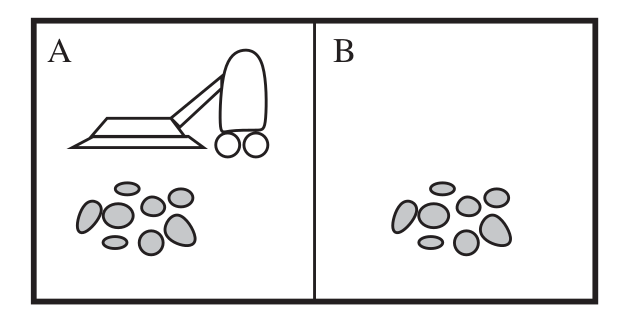
\includegraphics[width=0.7\textwidth]{figs/aspirador.png}
 \caption{Mundo do aspirador: dois quadrados, cada um limpo ou sujo.}
 \end{figure}
\end{frame}

\begin{frame}
\frametitle{Exemplo: Agente Aspirador de Pó}
\begin{itemize}
    \item O agente aspirador limpa o quadrado onde está se ele estiver sujo, e se move para o outro quadrado caso contrário.
    \item A função do agente pode ser inteiramente descrita por uma tabela que mapeia cada percepção possível (local + estado) na ação correspondente.
\end{itemize}
\begin{figure}
 \centering
 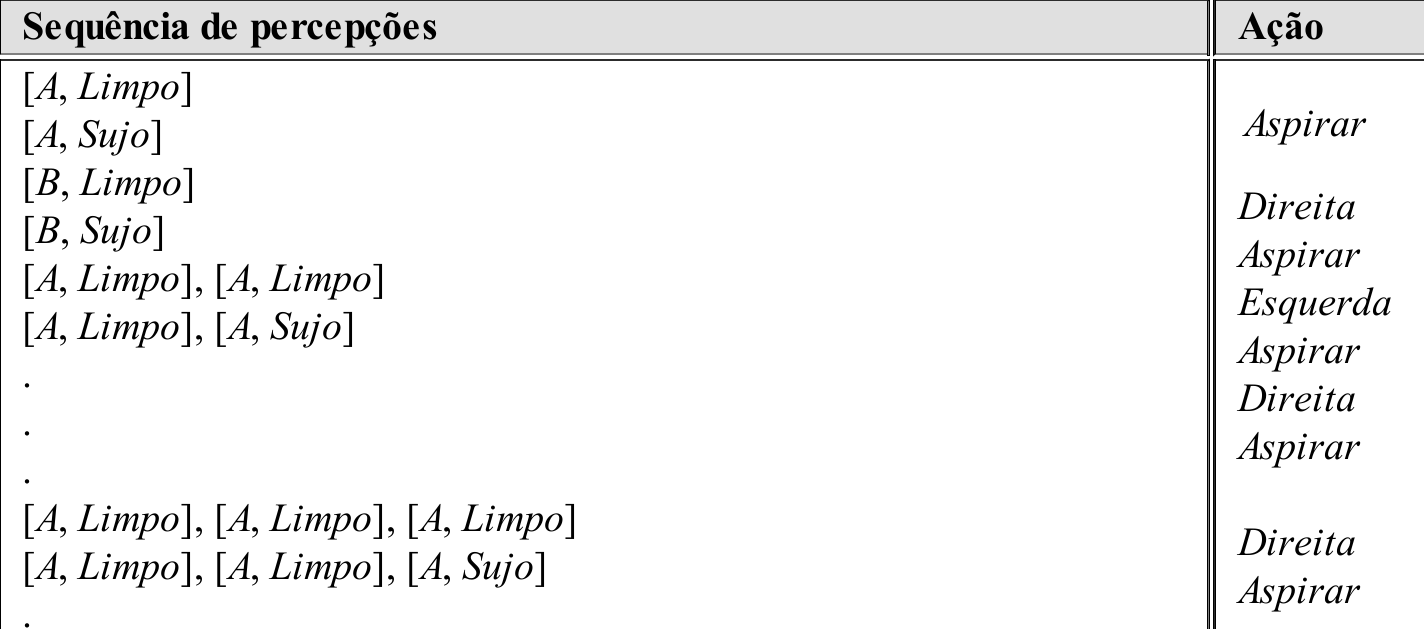
\includegraphics[width=0.65\textwidth]{figs/percepcao.png}
\caption{Tabela parcial da função de um agente simples no mundo do aspirador de pó.}
 \end{figure}
\end{frame}

\begin{frame}
\frametitle{Medida de Desempenho}
\footnotesize
\begin{itemize}
    \item É o critério objetivo usado para avaliar \textit{o quão bem} o agente se saiu. Não existe uma medida universal: ela precisa ser definida para cada ambiente e objetivo.
    \item Exemplo: no mundo do aspirador, poderia ser a quantidade de sujeira removida, o tempo gasto ou a energia consumida ao longo de 1000 passos.
\end{itemize}
\begin{block}{Princípio de projeto}
\textit{De modo geral, é melhor definir a medida de desempenho em função do \textbf{resultado desejado no ambiente} (``casa limpa'') do que em função do \textbf{comportamento esperado do agente} (``aspirar sempre que possível''), pois a segunda abordagem pode recompensar um agente que age bem sem de fato atingir o objetivo.}
\end{block}
\end{frame}

\begin{frame}
\frametitle{Racionalidade do Agente: Quatro Fatores}
\footnotesize
\begin{itemize}
    \item A racionalidade de uma ação, em um dado instante, depende de quatro fatores:
    \begin{itemize}
        \item A \textbf{medida de desempenho} que define o critério de sucesso.
        \item O \textbf{conhecimento prévio} do agente sobre o ambiente.
        \item As \textbf{ações} que o agente pode realizar.
        \item A \textbf{sequência de percepções} que o agente teve até o momento.
    \end{itemize}
\end{itemize}
\begin{block}{Definição de agente racional}
\textit{Para cada sequência de percepções possível, um agente racional deve escolher uma ação que maximize sua medida de desempenho esperada, dadas as evidências fornecidas pela sequência de percepções e todo o conhecimento prévio do agente.}
\end{block}
\end{frame}

\begin{frame}
\frametitle{Racionalidade e Otimalidade}
\begin{itemize}
    \item \textbf{Racionalidade} maximiza o desempenho \textit{esperado}, com base no que o agente sabe no momento da decisão.
    \item \textbf{Otimalidade} exigiria maximizar o desempenho \textit{real}, considerando toda informação relevante, inclusive a que o agente não tem como possuir.
    \item Por isso racionalidade e otimalidade nem sempre coincidem: limitações de tempo, conhecimento e capacidade computacional impedem que um agente seja perfeito, mas não impedem que ele seja racional.
\end{itemize}
\end{frame}

\begin{frame}
\frametitle{Conhecimento Prévio}
\begin{itemize}
    \item O que o agente sabe sobre o ambiente antes de começar a operar.
    \item Inclui modelos do ambiente, regras de interação, e experiências passadas.
    \item Exemplo: Um agente de navegação pode conhecer a disposição das ruas, mas não as condições de tráfego em tempo real.
\end{itemize}
\end{frame}

\begin{frame}
\frametitle{Ações Possíveis}
\begin{itemize}
    \item As ações que o agente pode realizar em resposta às percepções.
    \item A racionalidade de um agente inclui considerar todas as ações possíveis e escolher a melhor delas.
    \item Exemplo: Um robô móvel pode escolher entre avançar, virar ou parar com base nas percepções de seu sensor.
\end{itemize}
\end{frame}

\begin{frame}
\frametitle{Sequência de Percepções}
\begin{itemize}
    \item A sequência de percepções passadas pode influenciar as decisões futuras do agente.
    \item Um agente racional utiliza essa sequência para atualizar seu conhecimento e refinar suas decisões.
    \item Exemplo: Um agente de investimento pode ajustar sua estratégia com base em padrões observados no mercado.
\end{itemize}
\end{frame}

\subsection{Onisciência}
\begin{frame}
\frametitle{Racionalidade não é Onisciência}
\begin{itemize}
    \item Um agente \textbf{racional} escolhe a melhor ação com base no que percebeu e sabe, e não no que \textit{acabaria} acontecendo.
    \item Um agente \textbf{onisciente} conheceria o resultado real de cada ação de antemão. Isso simplesmente não existe no mundo real.
    \item Exemplo clássico: alguém atravessa a rua numa faixa segura e, por puro azar, é atingido por uma peça que cai de um avião. A decisão de atravessar continua racional, pois não havia como prever aquele evento com a informação disponível.
\end{itemize}
\end{frame}

\begin{frame}
\frametitle{Perfeição vs. Racionalidade}
\begin{itemize}
    \item Racionalidade maximiza o desempenho \textit{esperado}, enquanto a perfeição exigiria maximizar o desempenho \textit{real}, incluindo eventos impossíveis de antecipar.
    \item Exigir perfeição tornaria o projeto de agentes práticos inviável, já que nenhum sistema real consegue prever todos os desdobramentos futuros de suas ações.
\end{itemize}
\end{frame}

\begin{frame}
\frametitle{Aprendizado e Autonomia}
\begin{itemize}
    \item \textbf{Aprendizado}: um agente racional deve conseguir melhorar seu desempenho ao longo do tempo, ajustando-se com base no que observa.
    \item \textbf{Autonomia}: um agente deve agir cada vez mais a partir da própria experiência, e não apenas do conhecimento que lhe foi programado de antemão.
    \item Exemplo: um robô de limpeza que nunca viu o ambiente consegue, explorando-o, descobrir sozinho onde a sujeira se acumula com mais frequência, e adaptar sua rota de acordo.
\end{itemize}
\end{frame}


\subsection{Natureza dos ambientes}
\begin{frame}
\frametitle{Definição do Ambiente de Tarefa}
\begin{itemize}
    \item O ambiente de tarefa de um agente inclui todos os aspectos externos ao agente que são relevantes para a definição do problema que ele deve resolver.
    \begin{itemize}
     \item Ao projetar um agente, a primeira etapa deve ser sempre especificar o ambiente de tarefa chamado de \textbf{PEAS}
    \end{itemize}
    \item \textbf{PEAS}:
    \begin{itemize}
        \item P: Performance Measure (Medida de Desempenho)
        \item E: Environment (Ambiente)
        \item A: Actuators (Atuadores)
        \item S: Sensors (Sensores)
    \end{itemize}
\end{itemize}
\end{frame}

\begin{frame}
\frametitle{Exemplo de PEAS: Agente Aspirador de Pó}
\begin{itemize}
    \item Medida de Desempenho: Quantidade de sujeira removida, tempo gasto, energia consumida.
    \item Ambiente: Ambiente doméstico com áreas limpas e sujas.
    \item Atuadores: Motores de movimentação e sistema de sucção.
    \item Sensores: Sensores de sujeira, sensores de parede, sensores de localização.
\end{itemize}

\end{frame}

\begin{frame}
\frametitle{PEAS: Agente de Condução Autônoma (ex: Uber)}
\begin{center}
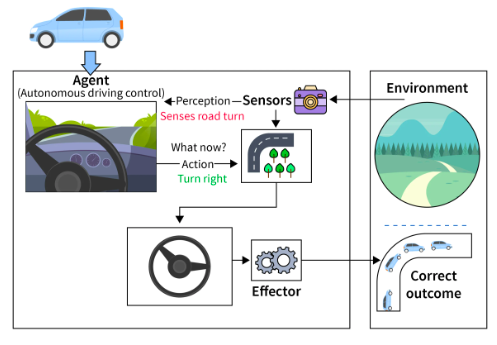
\includegraphics[width=0.52\textwidth]{figs/ambiente_agente.png}
\end{center}
\vspace{4pt}
\begin{center}
\footnotesize
\begin{tabular}{@{}p{0.9cm}p{8.3cm}@{}}
\toprule
\textbf{P} & Segurança, conformidade com as regras de trânsito, eficiência \\
\textbf{E} & Ruas, outros veículos, pedestres, sinais de trânsito \\
\textbf{A} & Motores, volante, freios \\
\textbf{S} & Câmeras, radar, GPS, sensores de velocidade \\
\bottomrule
\end{tabular}
\end{center}
\end{frame}

\begin{frame}
\frametitle{PEAS para Diferentes Ambientes}
\footnotesize
\begin{itemize}
    \item Agente de Diagnóstico Médico:
    \begin{itemize}
        \item P: Precisão do diagnóstico, tempo de resposta.
        \item E: Histórico do paciente, sintomas apresentados, resultados de exames.
        \item A: Interface de comunicação, recomendações de tratamento.
        \item S: Entrada de dados de sintomas, resultados laboratoriais.
    \end{itemize}
\end{itemize}
\end{frame}

\begin{frame}
\frametitle{Tabela de Exemplos de PEAS}
\begin{table}[h!]
\centering
\tiny
\begin{tabular}{@{}p{1.9cm}p{1.4cm}p{1.4cm}p{1.9cm}p{1.9cm}@{}}
\toprule
\textbf{Agente} & \textbf{P} & \textbf{E} & \textbf{A} & \textbf{S} \\
\midrule
Aspirador de Pó & Limpeza & Casa & Motores, sucção & Sensores de sujeira \\
Condução Autônoma & Segurança & Ruas & Volante, freios & Câmeras, radar \\
Diagnóstico Médico & Precisão & Clínicas & Recomendações & Entrada de dados \\
\textit{Robô de Entrega de Pacotes} & \textit{?} & \textit{?} & \textit{?} & \textit{?} \\
\bottomrule
\end{tabular}
\caption{\scriptsize Exemplos de PEAS, cuja última linha é o exercício a seguir.}
\end{table}
\end{frame}


\begin{frame}
\frametitle{Especificando o Ambiente de Tarefa}
\begin{itemize}
    \item A especificação clara do ambiente de tarefa é crucial para o design e a implementação de agentes racionais.
    \item Compreender os componentes do PEAS ajuda a definir os requisitos e as restrições de cada agente.
    \item Impacta diretamente na escolha de algoritmos e na arquitetura do agente.
\end{itemize}
\end{frame}


\begin{frame}
\frametitle{Tarefa 1: Robô de Entrega de Pacotes na UFPA de Cametá}
Imagine que você está desenvolvendo um robô autônomo capaz de entregar pacotes em um campus universitário. O robô deve navegar pelos prédios, evitar obstáculos, e garantir que os pacotes sejam entregues no local certo.
\end{frame}

\begin{frame}
\frametitle{Questão 1: Medida de Desempenho (Performance Measure)}
\begin{itemize}
    \item Como você definiria a medida de desempenho para este robô de entrega?
    \item Quais métricas devem ser usadas para avaliar se o robô está executando bem sua tarefa?
\end{itemize}
\end{frame}

\begin{frame}
\frametitle{Questão 2: Ambiente (Environment)}
\begin{itemize}
    \item Descreva o ambiente no qual o robô operará.
    \item Quais são os elementos do ambiente que o robô precisará considerar ao tomar decisões?
\end{itemize}

\end{frame}

\begin{frame}
\frametitle{Questão 3: Atuadores (Actuators)}
\begin{itemize}
    \item Quais atuadores o robô precisará para realizar suas ações?
    \item Considere todos os tipos de movimentos e interações que o robô terá com o ambiente.
\end{itemize}
\end{frame}

\begin{frame}
\frametitle{Questão 4: Sensores (Sensors)}
\begin{itemize}
    \item Quais sensores o robô precisará para perceber o ambiente e tomar decisões informadas?
    \item Considere tanto sensores para navegação quanto para interação com os objetos e pessoas.
\end{itemize}
\end{frame}


\begin{frame}
\frametitle{Solução: PEAS do Robô de Entrega de Pacotes}
\begin{table}[h!]
\centering
\scriptsize
\begin{tabular}{@{}p{2.5cm}p{7.8cm}@{}}
\toprule
\textbf{P} & Pacotes entregues no prazo e no local certo, sem danos, tempo total gasto e energia consumida. \\
\textbf{E} & Prédios, corredores, rampas, elevadores, pessoas e outros obstáculos do campus. \\
\textbf{A} & Motores de locomoção, braço ou compartimento para soltar o pacote, display/alto-falante para interagir com pessoas. \\
\textbf{S} & Câmeras, LiDAR ou sonares para navegação, GPS/mapa interno, leitor de código do pacote, sensores de contato/colisão. \\
\bottomrule
\end{tabular}
\caption{Uma resposta possível: compare com a sua.}
\end{table}
\end{frame}


\subsection{Propriedades de ambientes de
tarefas}
\begin{frame}
\frametitle{Propriedades dos Ambientes de Tarefa}
\begin{itemize}
    \item Depois de especificar o PEAS, o próximo passo é caracterizar o \textbf{ambiente} segundo um conjunto de dimensões, pois isso é o que realmente determina qual algoritmo e qual arquitetura de agente fazem sentido.
    \item As seis dimensões a seguir formam um ``checklist'' que vale a pena aplicar a qualquer ambiente novo que vocês encontrarem.
\end{itemize}
\end{frame}

\begin{frame}
\frametitle{Totalmente Observável vs. Parcialmente Observável}
\begin{itemize}
    \item \textbf{Totalmente observável}: os sensores do agente dão acesso ao estado completo do ambiente, relevante para a decisão, a cada instante.
    \item \textbf{Parcialmente observável}: a informação é incompleta, ruidosa ou simplesmente inacessível (sensores limitados, ambiente oculto).
\end{itemize}
\comparediagram{\faChess}{Totalmente Observável}{Xadrez: o tabuleiro inteiro está sempre visível}{\faSmog}{Parcialmente Observável}{Dirigir na neblina: só se vê um pedaço da pista}{blue}{orange}
\end{frame}

\begin{frame}
\frametitle{Determinístico vs. Estocástico}
\begin{itemize}
    \item \textbf{Determinístico}: o próximo estado é inteiramente definido pelo estado atual e pela ação do agente, sem acaso envolvido.
    \item \textbf{Estocástico}: há incerteza genuína no resultado da ação, de modo que o próximo estado segue uma distribuição de \textbf{probabilidades}.
\end{itemize}
\comparediagram{\faChess}{Determinístico}{Xadrez: a jogada define o novo estado}{\faCloudSunRain}{Estocástico}{Previsão do tempo: o resultado é incerto}{blue}{orange}
\end{frame}

\begin{frame}
\frametitle{Episódico vs. Sequencial}
\begin{itemize}
    \item \textbf{Episódico}: a experiência do agente é dividida em episódios independentes, de modo que a decisão de um episódio não afeta os seguintes.
    \item \textbf{Sequencial}: a decisão atual pode afetar todas as decisões futuras, exigindo pensar à frente.
\end{itemize}
\comparediagram{\faImage}{Episódico}{Classificar uma imagem por vez, sem memória do que veio antes}{\faCarSide}{Sequencial}{Dirigir: cada manobra afeta as próximas}{blue}{orange}
\end{frame}

\begin{frame}
\frametitle{Estático vs. Dinâmico}
\begin{itemize}
    \item \textbf{Estático}: o ambiente permanece parado enquanto o agente delibera, de modo que não há pressa em decidir.
    \item \textbf{Dinâmico}: o ambiente pode mudar durante a deliberação do agente, que precisa decidir em tempo hábil.
\end{itemize}
\comparediagram{\faPuzzlePiece}{Estático}{Quebra-cabeça: espera o tempo que for preciso}{\faFutbol}{Dinâmico}{Futebol: a bola não espera o agente pensar}{blue}{orange}
\end{frame}

\begin{frame}
\frametitle{Discreto vs. Contínuo}
\begin{itemize}
    \item \textbf{Discreto}: número finito (e geralmente pequeno) de estados, percepções e ações distintas.
    \item \textbf{Contínuo}: estados, tempo ou ações variam em um espaço contínuo, potencialmente infinito.
\end{itemize}
\comparediagram{\faThLarge}{Discreto}{Jogo de tabuleiro: casas e movimentos bem definidos}{\faRobot}{Contínuo}{Controle de um robô móvel: posição e velocidade variam continuamente}{blue}{orange}
\end{frame}

\begin{frame}
\frametitle{Agente Único vs. Multiagente}
\begin{itemize}
    \item \textbf{Agente único}: o agente opera sozinho, e o ambiente não contém outros agentes tomando decisões.
    \item \textbf{Multiagente}: outros agentes atuam no mesmo ambiente, de forma cooperativa (um time) ou competitiva (um adversário).
\end{itemize}
\comparediagram{\faPuzzlePiece}{Agente Único}{Resolver um quebra-cabeça sozinho}{\faUsers}{Multiagente}{Jogar xadrez contra um oponente}{blue}{orange}
\end{frame}

\begin{frame}
\frametitle{Outras Propriedades}
\begin{itemize}
    \item \textbf{Conhecido vs. Desconhecido}: um ambiente é conhecido quando o agente já sabe, de antemão, como suas ações afetam o ambiente (as ``regras do jogo''), e é desconhecido quando o agente precisa explorar para aprender essas regras.
    \item Essa dimensão é diferente de observabilidade: é possível ter um ambiente totalmente observável e, ainda assim, desconhecido (por exemplo, um jogo novo cujas regras exatas não foram explicadas).
    \item Exemplo: Jogo de xadrez para um jogador experiente (conhecido) vs. explorar a superfície de Marte pela primeira vez (desconhecido).
\end{itemize}
\end{frame}

\begin{frame}
\frametitle{Impacto no Design de Agentes}
\begin{itemize}
    \item Cada dimensão empurra o projeto do agente em uma direção: ambientes parcialmente observáveis exigem manter algum estado interno, ambientes dinâmicos exigem decisões rápidas e ambientes estocásticos exigem raciocinar sobre probabilidades.
    \item \textbf{O caso mais difícil} combina tudo de uma vez: \textbf{parcialmente observável, multiagente, estocástico, sequencial, dinâmico, contínuo e desconhecido}.
    \begin{itemize}
     \item Exemplo: dirigir em um país desconhecido, com geografia, leis de trânsito e comportamento dos outros motoristas que o agente ainda não domina.
    \end{itemize}
    \item Boa parte da pesquisa em IA existe justamente para lidar com combinações difíceis como essa, e é o que veremos nas próximas aulas.
\end{itemize}
\end{frame}

\subsection{Estrutura de Agente}

\begin{frame}
\frametitle{Arquitetura e Programa de Agentes}
\footnotesize
\begin{itemize}
    \item O trabalho da IA é projetar um \textbf{programa de agente}: o algoritmo que implementa a função do agente, mapeando percepções em ações.
    \item Esse programa roda sobre uma \textbf{arquitetura}, o dispositivo físico com sensores e atuadores (um PC, um carro robótico, um celular).
\end{itemize}
\begin{center}
\textbf{agente = arquitetura + programa}
\end{center}
\begin{itemize}
    \item O programa precisa ser compatível com a arquitetura: se ele recomenda a ação ``andar'', a arquitetura precisa ter pernas.
\end{itemize}
\end{frame}

\begin{frame}
\frametitle{O que é um Programa de Agente}
\footnotesize
\begin{itemize}
    \item É o algoritmo que recebe a percepção atual como entrada e devolve uma ação, a cada ciclo de execução do agente.
    \item Note a diferença: a \textbf{função} do agente é uma descrição matemática abstrata ($f: P^* \rightarrow A$), enquanto o \textbf{programa} é a implementação concreta que roda na arquitetura.
\end{itemize}
\begin{center}
\begin{tikzpicture}[scale=0.85, every node/.style={transform shape, font=\scriptsize, align=center}, node distance=6mm and 9mm]
  \node[circle, draw, thick, minimum size=0.9cm] (sensor) {Sensores};
  \node[draw, thick, rounded corners, minimum width=2.6cm, minimum height=0.9cm, right=of sensor] (prog) {Programa\\de Agente};
  \node[circle, draw, thick, minimum size=0.9cm, right=of prog] (atuador) {Atuadores};
  \draw[-{Latex[length=2mm]}, thick] (sensor) -- node[above, font=\tiny] {percepção} (prog);
  \draw[-{Latex[length=2mm]}, thick] (prog) -- node[above, font=\tiny] {ação} (atuador);
\end{tikzpicture}
\end{center}
\end{frame}

\begin{frame}[fragile]
\frametitle{Pseudocódigo: Agente Dirigido por Tabela}
\small
\begin{itemize}
    \item A implementação mais direta de um programa de agente é uma \textbf{tabela}: para cada sequência de percepções já vista, uma ação associada.
\end{itemize}
\begin{verbatim}
function TABLE-DRIVEN-AGENT(percept) returns action
  persistent: percepts, uma lista, inicialmente vazia
              table, uma tabela de ações, indexada por
                     sequências de percepções

  append percept ao final de percepts
  action <- LOOKUP(percepts, table)
  return action
\end{verbatim}
\begin{itemize}
    \item \textbf{Limitação séria}: a tabela cresce exponencialmente com o número de percepções possíveis, tornando essa abordagem inviável na prática para a maioria dos ambientes.
\end{itemize}
\end{frame}

\begin{frame}
\frametitle{Tipos de Programas de Agentes}
\begin{itemize}
    \item Existem quatro famílias clássicas de programas de agentes, em ordem crescente de complexidade e de capacidade de lidar com ambientes difíceis:
    \begin{itemize}
        \item \textbf{Reflexo simples}: decide com base só na percepção atual.
        \item \textbf{Baseado em modelo}: mantém um estado interno sobre o que não pode observar diretamente.
        \item \textbf{Baseado em objetivos}: decide prevendo se a ação aproxima do objetivo.
        \item \textbf{Baseado em utilidade}: decide comparando o quão \textit{bom} é cada resultado possível, não só se ele atinge o objetivo.
    \end{itemize}
\end{itemize}
\end{frame}

\begin{frame}
\frametitle{Agentes Simples de Reflexo}
\footnotesize
\begin{itemize}
    \item Escolhem a ação com base apenas na percepção atual, por meio de \textbf{regras condição-ação} (``se sujo, aspire'').
    \item Funcionam bem apenas quando o ambiente é \textbf{totalmente observável}: a decisão correta precisa depender só do que está sendo percebido agora.
    \item Limitação: sem memória do passado, podem entrar em loops em ambientes parcialmente observáveis (ex: ficar alternando entre dois estados). Uma saída parcial é introduzir \textbf{aleatoriedade} nas escolhas.
\end{itemize}
\begin{center}
\begin{tikzpicture}[scale=0.82, every node/.style={transform shape, font=\scriptsize, align=center}, node distance=5mm and 7mm]
  \node[circle, draw, thick, minimum size=0.85cm] (sensor) {Sensores};
  \node[draw, thick, rounded corners, minimum width=2.1cm, minimum height=0.8cm, right=of sensor] (mundo) {Como é o\\mundo agora};
  \node[draw, thick, rounded corners, minimum width=2.1cm, minimum height=0.8cm, right=of mundo] (acao) {Qual ação\\tomar agora};
  \node[circle, draw, thick, minimum size=0.85cm, right=of acao] (atuador) {Atuadores};
  \node[draw, thick, rounded corners=6pt, fill=orange!10, minimum width=2.3cm, minimum height=0.7cm, below=0.5cm of acao] (regras) {Regras\\condição-ação};
  \draw[-{Latex[length=2mm]}, thick] (sensor) -- (mundo);
  \draw[-{Latex[length=2mm]}, thick] (mundo) -- (acao);
  \draw[-{Latex[length=2mm]}, thick] (acao) -- (atuador);
  \draw[-{Latex[length=2mm]}, thick] (regras) -- (acao);
\end{tikzpicture}
\end{center}
\end{frame}

\begin{frame}[fragile]
\frametitle{Pseudocódigo: Agente de Reflexo Simples}
\small
\begin{itemize}
    \item Exemplo no mundo do aspirador: a ação depende só de onde o agente está e se o local está sujo.
\end{itemize}
\begin{verbatim}
function REFLEX-AGENT(location, status) returns action
  if status = SUJO then return ASPIRAR
  else if location = A then return DIREITA
  else if location = B then return ESQUERDA
\end{verbatim}
\end{frame}

\begin{frame}
\frametitle{Agentes Baseados em Modelo}
\footnotesize
\begin{itemize}
    \item Mantêm um \textbf{estado interno} que guarda parte do histórico, combinado com um \textbf{modelo} de como o mundo evolui e do efeito das próprias ações.
    \item São mais robustos que os de reflexo simples: conseguem agir mesmo quando a percepção atual, sozinha, não basta para decidir.
\end{itemize}
\begin{center}
\begin{tikzpicture}[scale=0.8, every node/.style={transform shape, font=\scriptsize, align=center}, node distance=5mm and 7mm]
  \node[circle, draw, thick, minimum size=0.8cm] (sensor) {Sensores};
  \node[draw, thick, rounded corners, minimum width=2.1cm, minimum height=0.8cm, right=of sensor] (mundo) {Como é o\\mundo agora};
  \node[draw, thick, rounded corners, minimum width=2.1cm, minimum height=0.8cm, right=of mundo] (acao) {Qual ação\\tomar agora};
  \node[circle, draw, thick, minimum size=0.8cm, right=of acao] (atuador) {Atuadores};
  \node[draw, thick, rounded corners=6pt, fill=orange!10, minimum width=2.3cm, minimum height=0.6cm, below=0.4cm of acao] (regras) {Regras\\condição-ação};
  \node[draw, thick, rounded corners=6pt, fill=teal!10, minimum width=2.3cm, minimum height=0.7cm, above=0.4cm of mundo] (modelo) {Modelo: como o mundo\\evolui e efeito das ações};
  \node[draw, thick, rounded corners=6pt, fill=teal!10, minimum width=1.6cm, minimum height=0.6cm, above=0.4cm of modelo] (estado) {Estado};
  \draw[-{Latex[length=2mm]}, thick] (sensor) -- (mundo);
  \draw[-{Latex[length=2mm]}, thick] (mundo) -- (acao);
  \draw[-{Latex[length=2mm]}, thick] (acao) -- (atuador);
  \draw[-{Latex[length=2mm]}, thick] (regras) -- (acao);
  \draw[-{Latex[length=2mm]}, thick] (estado) -- (modelo);
  \draw[-{Latex[length=2mm]}, thick] (modelo) -- (mundo);
\end{tikzpicture}
\end{center}
\end{frame}

\begin{frame}
\frametitle{Modelo do Ambiente}
Um agente baseado em modelo mantém, internamente, uma função que descreve a transição de estados:
\[
M: S \times A \rightarrow S
\]
onde \( S \) é o conjunto de estados possíveis do ambiente e \( A \) é o conjunto de ações do agente.
\end{frame}

\begin{frame}[fragile]
\frametitle{Pseudocódigo: Agente de Reflexo com Modelo}
\footnotesize
\begin{verbatim}
function MODEL-BASED-REFLEX-AGENT(percept) returns action
  persistent: state,  a concepção atual do agente sobre o mundo
              model,  como o próximo estado depende de
                      estado e ação
              rules,  um conjunto de regras condição-ação
              action, a última ação, inicialmente nenhuma

  state <- UPDATE-STATE(state, action, percept, model)
  rule  <- RULE-MATCH(state, rules)
  action <- rule.ACTION
  return action
\end{verbatim}
\end{frame}

\begin{frame}
\frametitle{Agentes Baseados em Objetivos}
\footnotesize
\begin{itemize}
    \item Além do estado atual, consideram um \textbf{objetivo}: o estado que desejam alcançar. A ação escolhida é a que aproxima desse objetivo, não apenas a reação imediata.
    \item Exemplo: um robô de entrega decide a melhor \textbf{rota} até o destino, em vez de apenas reagir ao obstáculo mais próximo.
    \item Para isso, costumam usar \textbf{algoritmos de busca e planejamento} (assunto de aulas futuras).
\end{itemize}
\[
G(s) = \begin{cases}
1 & \text{se } s \text{ é um estado objetivo} \\
0 & \text{caso contrário}
\end{cases}
\]
\begin{center}
\begin{tikzpicture}[scale=0.82, every node/.style={transform shape, font=\scriptsize, align=center}, node distance=5mm and 7mm]
  \node[circle, draw, thick, minimum size=0.85cm] (sensor) {Sensores};
  \node[draw, thick, rounded corners, minimum width=2.1cm, minimum height=0.8cm, right=of sensor] (mundo) {Como é o\\mundo agora};
  \node[draw, thick, rounded corners, minimum width=2.1cm, minimum height=0.8cm, right=of mundo] (acao) {Qual ação\\aproxima do objetivo};
  \node[circle, draw, thick, minimum size=0.85cm, right=of acao] (atuador) {Atuadores};
  \node[draw, thick, rounded corners=6pt, fill=orange!10, minimum width=2.1cm, minimum height=0.7cm, below=0.5cm of acao] (objetivos) {Objetivos\\\( G(s) \)};
  \draw[-{Latex[length=2mm]}, thick] (sensor) -- (mundo);
  \draw[-{Latex[length=2mm]}, thick] (mundo) -- (acao);
  \draw[-{Latex[length=2mm]}, thick] (acao) -- (atuador);
  \draw[-{Latex[length=2mm]}, thick] (objetivos) -- (acao);
\end{tikzpicture}
\end{center}
\end{frame}

\begin{frame}[fragile]
\frametitle{Pseudocódigo: Busca em Largura (BFS)}
\footnotesize
\begin{itemize}
    \item Exemplo clássico de algoritmo usado por agentes baseados em objetivos para encontrar um caminho até a meta:
\end{itemize}
\begin{verbatim}
function BFS(start, goal) returns a path
  frontier <- fila com [start]
  explored <- conjunto vazio

  while frontier não está vazia:
    node <- frontier.pop()
    if node = goal then return solution

    for each neighbor in node.neighbors:
      if neighbor not in explored:
        frontier.push(neighbor)
        explored.add(neighbor)
\end{verbatim}
\end{frame}

\begin{frame}
\frametitle{Vantagens e Limitações}
\footnotesize
\begin{itemize}
    \item \textbf{Vantagens}: mais flexíveis que o reflexo simples, planejam à frente e consideram várias alternativas antes de agir.
    \item \textbf{Limitações}: a busca pela solução ideal pode exigir muito poder computacional, prever resultados é difícil em ambientes estocásticos, e os planos precisam ser atualizados quando o ambiente muda.
\end{itemize}
\end{frame}

\begin{frame}
\frametitle{Agentes Baseados em Utilidade}
\footnotesize
\begin{itemize}
    \item Vão além de um objetivo binário (``atingi ou não atingi''): avaliam o quão \textbf{bom} é cada estado possível, por meio de uma \textbf{função de utilidade}.
    \item Útil quando há vários objetivos conflitantes (rapidez vs. segurança) ou resultados incertos a comparar.
\end{itemize}
\[
U(s) = \sum_{i} w_i \cdot f_i(s)
\]
onde \( w_i \) são pesos e \( f_i(s) \) são características do estado \( s \).
\begin{center}
\begin{tikzpicture}[scale=0.82, every node/.style={transform shape, font=\scriptsize, align=center}, node distance=5mm and 7mm]
  \node[circle, draw, thick, minimum size=0.85cm] (sensor) {Sensores};
  \node[draw, thick, rounded corners, minimum width=2.1cm, minimum height=0.8cm, right=of sensor] (mundo) {Como é o\\mundo agora};
  \node[draw, thick, rounded corners, minimum width=2.1cm, minimum height=0.8cm, right=of mundo] (acao) {Qual ação\\maximiza utilidade};
  \node[circle, draw, thick, minimum size=0.85cm, right=of acao] (atuador) {Atuadores};
  \node[draw, thick, rounded corners=6pt, fill=orange!10, minimum width=2.1cm, minimum height=0.7cm, below=0.5cm of acao] (utilidade) {Utilidade\\\( U(s) \)};
  \draw[-{Latex[length=2mm]}, thick] (sensor) -- (mundo);
  \draw[-{Latex[length=2mm]}, thick] (mundo) -- (acao);
  \draw[-{Latex[length=2mm]}, thick] (acao) -- (atuador);
  \draw[-{Latex[length=2mm]}, thick] (utilidade) -- (acao);
\end{tikzpicture}
\end{center}
\end{frame}

\begin{frame}{Agentes de Aprendizado}
\footnotesize
\begin{itemize}
    \item Qualquer um dos quatro tipos anteriores pode virar um \textbf{agente de aprendizado}, ganhando a capacidade de melhorar com a experiência em vez de depender só de conhecimento pré-programado.
    \item Quatro componentes trabalham juntos: o \textbf{elemento de desempenho} escolhe as ações, o \textbf{crítico} avalia o resultado, o \textbf{elemento de aprendizado} ajusta o comportamento futuro, e o \textbf{gerador de problemas} sugere ações exploratórias para descobrir coisas novas.
\end{itemize}
\begin{center}
\begin{tikzpicture}[scale=0.78, every node/.style={transform shape, font=\scriptsize, align=center}, node distance=5mm and 9mm]
  \node[circle, draw, thick, minimum size=0.8cm] (sensor) {Sensores};
  \node[draw, thick, rounded corners, minimum width=2.4cm, minimum height=0.9cm, right=of sensor] (desempenho) {Elemento de\\Desempenho};
  \node[circle, draw, thick, minimum size=0.8cm, right=of desempenho] (atuador) {Atuadores};
  \node[draw, thick, rounded corners, fill=orange!10, minimum width=1.9cm, minimum height=0.7cm, above=of desempenho] (critico) {Crítico};
  \node[draw, thick, rounded corners, fill=orange!10, minimum width=2.1cm, minimum height=0.7cm, above=of critico] (aprendizado) {Elemento de\\Aprendizado};
  \node[draw, thick, rounded corners, fill=teal!10, minimum width=2.1cm, minimum height=0.7cm, left=of aprendizado] (gerador) {Gerador de\\Problemas};
  \draw[-{Latex[length=2mm]}, thick] (sensor) -- (desempenho);
  \draw[-{Latex[length=2mm]}, thick] (desempenho) -- (atuador);
  \draw[-{Latex[length=2mm]}, thick] (sensor) |- (critico);
  \draw[-{Latex[length=2mm]}, thick] (critico) -- (aprendizado);
  \draw[-{Latex[length=2mm]}, thick] (gerador) -- (aprendizado);
  \draw[-{Latex[length=2mm]}, thick, dashed] (aprendizado.east) to[out=0, in=90] node[midway, right, font=\tiny] {mudanças} (desempenho.north east);
\end{tikzpicture}
\end{center}
\end{frame}

\section{Implementação}
\subsection{Implementação de um agente}
\begin{frame}
\frametitle{Bibliotecas Clássicas para Agentes em Python}
\footnotesize
\begin{itemize}
    \item \textbf{AIMA-Python}: implementações de referência dos algoritmos e agentes do livro-texto do curso.
    \begin{itemize}
        \item \url{https://github.com/aimacode/aima-python}
    \end{itemize}
    \item \textbf{Mesa}: framework para simulação de agentes em ambientes 2D (modelagem baseada em agentes).
    \begin{itemize}
        \item \url{https://mesa.readthedocs.io/en/stable/}
    \end{itemize}
    \item \textbf{SPADE}: plataforma para agentes que se comunicam entre si pelo padrão FIPA, útil para sistemas multiagente.
    \begin{itemize}
        \item \url{https://github.com/javipalanca/spade}
    \end{itemize}
    \item \textbf{Gymnasium} (sucessor mantido do antigo OpenAI Gym): ambientes padronizados para treinar agentes com aprendizado por reforço.
    \begin{itemize}
        \item \url{https://gymnasium.farama.org/}
    \end{itemize}
\end{itemize}
\end{frame}

\begin{frame}
\frametitle{Da Teoria aos Agentes Baseados em LLM}
\footnotesize
\begin{itemize}
    \item As bibliotecas acima implementam a teoria clássica de agentes (AIMA). Hoje, uma nova geração de frameworks faz o mesmo papel usando um LLM como ``cérebro'' do agente.
    \item \textbf{LangChain} e \textbf{LangGraph}: orquestram o ciclo percepção-decisão-ação em torno de um LLM, dando a ele acesso a ferramentas, memória e fluxos de decisão com estado.
    \begin{itemize}
        \item \url{https://python.langchain.com/}
    \end{itemize}
    \item \textbf{Agno}: framework mais recente e leve, focado em agentes multiagente com memória, base de conhecimento e ferramentas prontas, com foco em velocidade de execução.
    \begin{itemize}
        \item \url{https://www.agno.com/}
    \end{itemize}
    \item Essas ferramentas serão exploradas em profundidade em aulas futuras desta disciplina, com exemplos práticos de agentes de IA em Python.
\end{itemize}
\end{frame}


\section{Referências Bibliográficas}
\begin{frame}[t,allowframebreaks]
\frametitle{Referências}
%\bibliographystyle{amsalpha}
%\bibliography{bibfile}
\begin{thebibliography}{*}

         \bibitem[A01]{A01} Chollet, F. (2021). Deep Learning with Python, Second Edition. Shelter Island, NY: Manning Publications.
        \bibitem[A02]{A02} Géron, A. (2019). Hands-On Machine Learning with Scikit-Learn, Keras, and TensorFlow. Sebastopol, CA: O'Reilly Media.
        \bibitem[A03]{A03} Russell, S., \& Norvig, P. (2021). Artificial Intelligence: A Modern Approach (4ª ed.). Hoboken, NJ: Pearson.
        \bibitem[A04]{A04} Moroney, L. (2020). AI and Machine Learning for Coders. Sebastopol, CA: O'Reilly Media.
        \bibitem[A05]{A05} Vaswani, A., et al. (2017). Attention Is All You Need. Advances in Neural Information Processing Systems (NeurIPS).

\end{thebibliography}
\end{frame}
\section{}

%remover logo
\setbeamertemplate{logo}{}

\begin{frame}
\titlepage
\end{frame}

\end{document}
